Los datos utilizados provienen de la competición Crowdsensing-based Road Damage Detection Challenge (CRDDC2022)\cite{CRDDC2022_paper}. Se trata de un conjunto de datos con imágenes de pavimentos, etiquetadas con la presencia de daños en el pavimento. Los datos provienen de seis países: China, República Checa, India, Japón, Noruega y Estados Unidos. Cada uno de estos países tiene un conjunto de datos que consiste en imágenes de carreteras tomadas desde un vehículo en movimiento. Además, China también proporciona un conjunto de datos con imágenes tomadas desde un dron, sumando un total de siete conjuntos de datos. Estos conjuntos de datos se dividen a su vez en entrenamiento y \textit{test}, donde el conjunto de entrenamiento se compone de imágenes con sus respectivas etiquetas de daños en el pavimento, y el conjunto de \textit{test} se compone de imágenes sin etiquetar. Las etiquetas de daños en el pavimento se proporcionan en forma de coordenadas de caja delimitadora y un identificador que representa el tipo de daño asociado a la caja.

Los organizadores de la competición han publicado un paper \cite{RDD2022_data_paper} donde se detallan los datos y se proporciona una descripción de los mismos. En esta sección se va a hacer un resumen de los datos y se va a explicar cómo están estructurados y que información contienen.


\subsubsection{¿Cómo descargar los datos?}
En el repositorio de la competición \cite{RoadDamageDetector_repo} se proporciona un fichero \textit{README} con una sección sobre los datos de la CRDDC2022. En esta sección del \textit{README} se pueden descargar \textit{zips} con los datos completos y por país. Además, se proporciona un enlace a \textit{figshare} \cite{RDD2022_dataset} donde se pueden descargar los datos completos. Personalmente, tuve problemas descargando los datos desde estas fuentes, ya que los datos correspondientes a Noruega estaban corruptos. Es por esto que opte por descargar los datos desde DatasetNinja \cite{RDD2022_datasetNinja}, donde se puede descargar los datos completos sin problemas.


\subsubsection{¿Cómo se estructuran los datos?}
Los datos de la CRDDC2022 se estructuran en siete carpetas, una por cada uno de los subconjuntos antes mencionados. Cada carpeta contiene dos carpetas, una de \textit{train} y otra de \textit{test}. Las carpetas de \textit{train} tienen otras dos subcarpetas una para las imágenes y otra para los archivos de anotaciones, mientras que las carpetas de \textit{test} solo tienen una carpeta de imágenes. Las imágenes y sus correspondientes anotaciones se nombran de la misma forma, de manera que se pueda asociar una imagen con su anotación. El formato de estos nombres es \texttt{<región>\_<identificador>.<extension>}, donde \texttt{<región>} es el subconjunto al que pertenece la imagen, \texttt{<identificador>} es un número que identifica a la imagen, y \texttt{<extension>} es la extensión del archivo. Las imágenes son todas en formato \texttt{jpg}, y las anotaciones son en formato \texttt{xml} si se descarga el conjunto por el repositorio de la competición o \textit{figshare}, y en formato \texttt{json} si se descarga el conjunto por DatasetNinja. En la descarga por DatasetNinja, los datos no están divididos por subconjunto, sino que se encuentran todos juntas en las carpetas generales de \textit{train} y \textit{test}.


\subsubsection{¿Cómo son las imágenes?}
Las imágenes han sido capturadas con sistemas muy diferentes dependiendo del subconjunto al que pertenecen. Esto junto con la diversidad de los entornos en los que se han tomado las imágenes, hace que las imágenes tengan una gran variabilidad en cuanto a calidad, resolución, iluminación, etc. En la tabla \ref{tab:dataset_info} se puede ver un resumen de la información sobre las imágenes de los datos de la CRDDC2022. En la figura \ref{fig:images_per_dataset_per_region} se muestra el número de imágenes de \textit{train} y \textit{test} por región en los datos de la CRDDC2022. Se observa que la cantidad de imágenes varía mucho entre regiones, con Japón teniendo una cantidad mucho mayor de imágenes en comparación con regiones como China o la República Checa. En la sección \ref{SEC:TRAIN} se explicará cómo puede afectar esto al ajuste de los modelos.

% Tabla explicativa de Region, Vehiculo, Dispositivo utilizado para capturar las imágenes, Resolución de las imágenes, Número de imágenes y Número de anotaciones
\begin{table}[H]
    \centering
    \resizebox{\textwidth}{!}{
        \begin{tabular}{|c|c|c|c|c|c|}
            \hline
            \textbf{Región} & \textbf{Vehículo} & \textbf{Dispositivo} & \textbf{Resolución} & \textbf{Nº Imágenes} & \textbf{Nº Anotaciones} \\
            \hline
            China & Motocicleta & Smartphone & 512x512 & 2477 & 4650 \\
            China & Dron (DJI M600 Pro) & Drone Camera & 512x512 & 2401 & 3068 \\
            República Checa & Vehículo & Dashcam & 600x600 & 3538 & 1745 \\
            India & Vehículo & Dashcam & 720x720 & 9665 & 6831 \\
            Japón & Vehículo & Dashcam & 600x600 & 13133 & 16470 \\
            Noruega & Vehículo & High-resolution Cameras & 4040x2035 & 10201 & 11229 \\
            Estados Unidos & Vehículo & Google Street View & 640x640 & 6005 & 11014 \\
            \hline
        \end{tabular}
    }
    \caption{Información sobre las imágenes de los datos de la CRDDC2022.}
    \label{tab:dataset_info}
\end{table}

% Añadimos las graficas de barras con el numero de imagenes para train y test por region (usamos subfigures)
\begin{figure}[H]
    \centering
    \subfigure[Número de imágenes de \textit{train} por región]{
        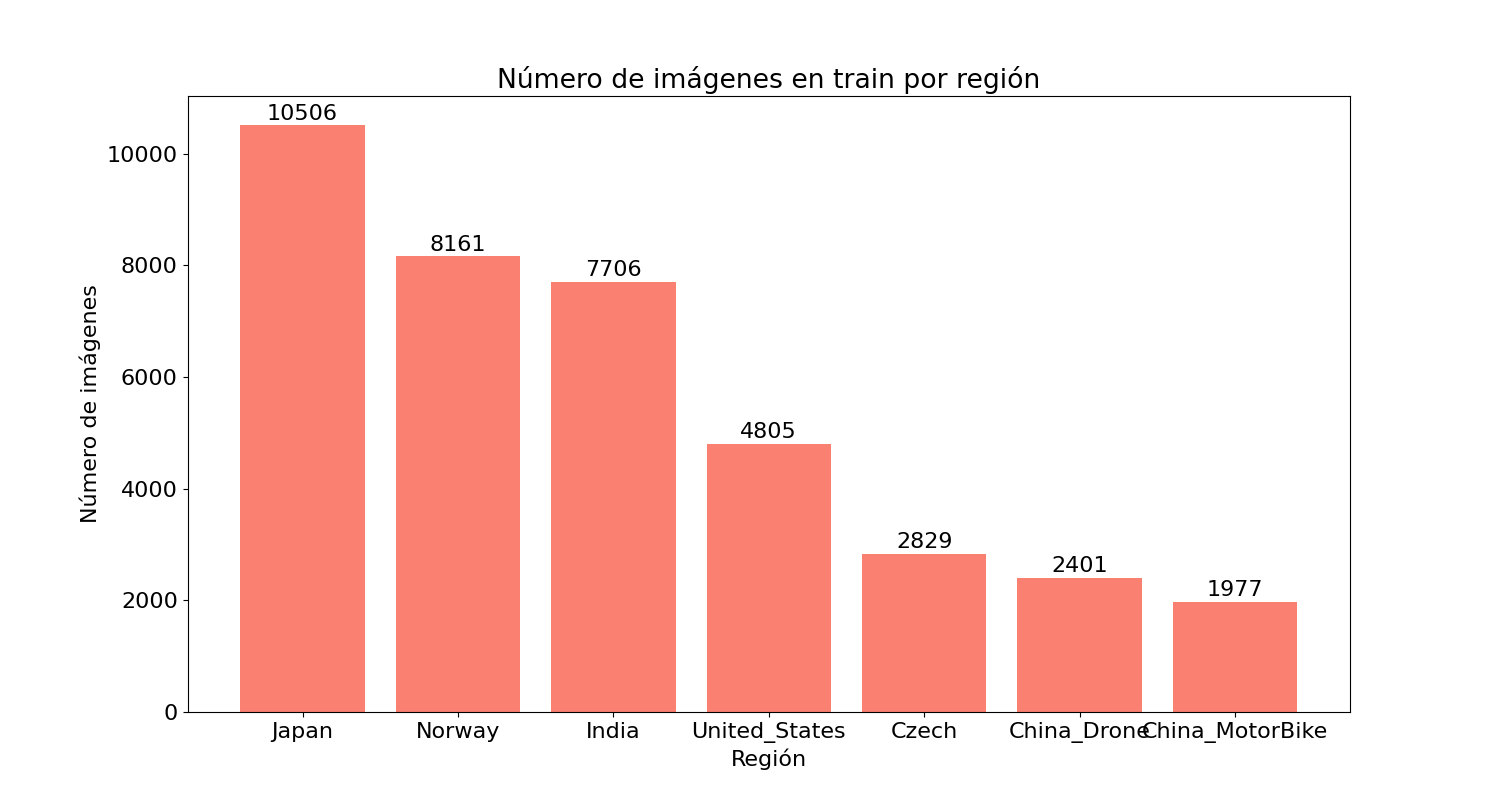
\includegraphics[width=0.45\textwidth]{../graphs/datasetNinja_train_images_per_region_bar.png}
        \label{fig:images_per_dataset_per_region_subfig1}
    }
    \subfigure[Número de imágenes de \textit{test} por región]{
        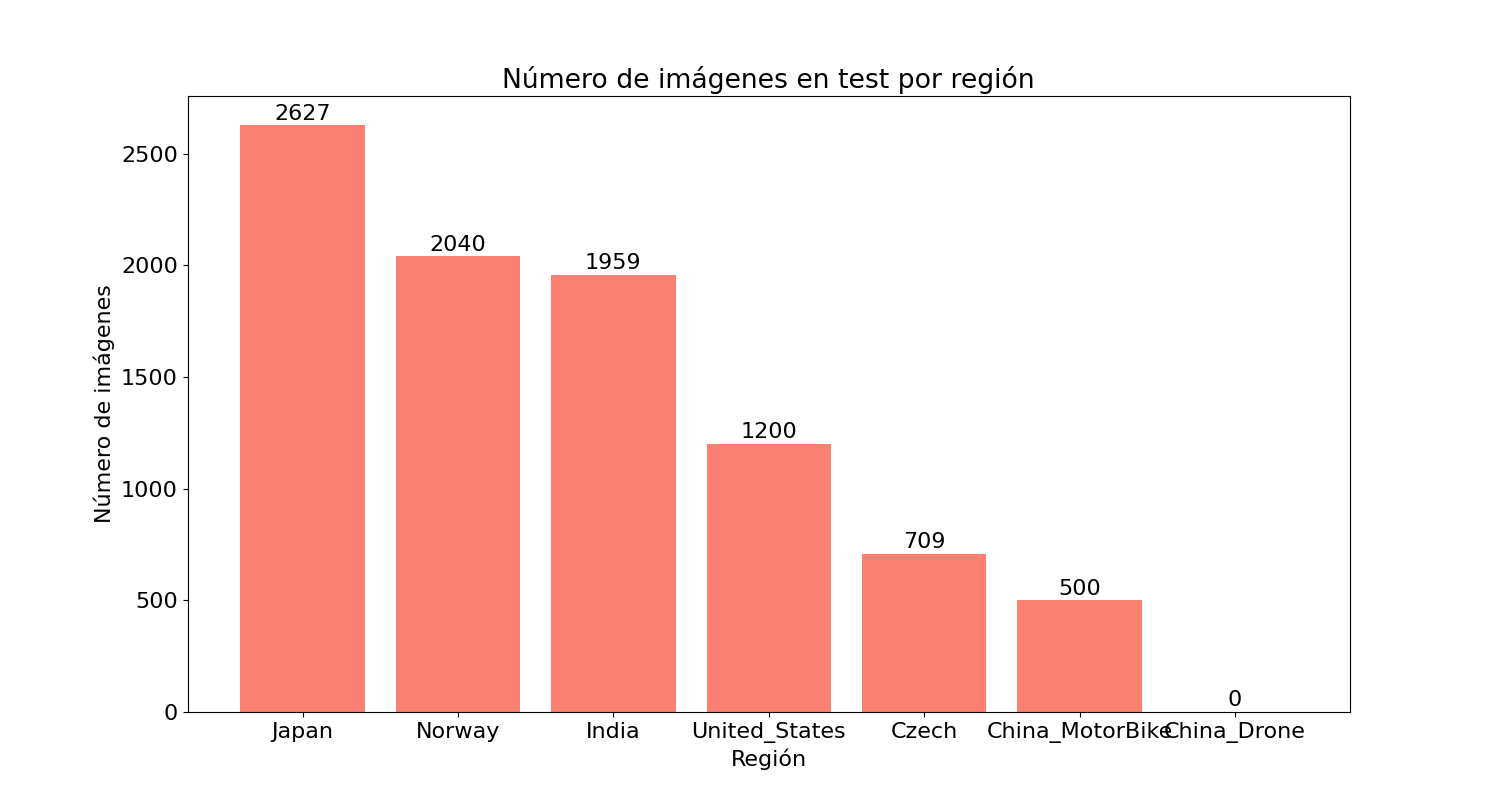
\includegraphics[width=0.45\textwidth]{../graphs/datasetNinja_test_images_per_region_bar.png}
        \label{fig:images_per_dataset_per_region_subfig2}
    }
    \caption{Número de imágenes de \textit{train} y \textit{test} por región en los datos de la CRDDC2022.}
    \label{fig:images_per_dataset_per_region}
\end{figure}

La resolución de las imágenes es un parámetro crucial, ya que afecta el tiempo de entrenamiento, la precisión, la complejidad y el tiempo de inferencia del modelo. Los modelos YOLO de Ultralytics redimensionan todas las imágenes antes de alimentarlas al modelo. Este redimensionado se controla con el parámetro \texttt{imgsz}, que se fija durante el entrenamiento del modelo. Todas las imágenes se redimensionan a \texttt{imgsz} en su lado más largo, manteniendo la relación de aspecto y añadiendo \textit{letterboxing}\footnote{Letterboxing es la técnica de redimensionar imágenes a otras dimensiones preservando la relación de aspecto mediante la adición de barras negras o grises para rellenar los espacios sobrantes.} cuando sea necesario. Para el entrenamiento de los modelos, he utilizado el \texttt{imgsz} predeterminado de Ultralytics, 640. En la tabla \ref{tab:dataset_info} se observa que las imágenes de Noruega tienen una resolución mucho mayor que esta resolución predeterminada. Por ello, he decidido redimensionar las imágenes de Noruega a un tamaño inferior, manteniendo la relación de aspecto, para reducir su tamaño en disco y facilitar su transferencia y almacenamiento. En la tabla \ref{tab:dataset_info} también se muestra una gran variabilidad en los métodos de captura de imagen. Debemos tener en cuenta esta variabilidad al entrenar nuestros modelos, ya que si no son capaces de generalizar bien, podrían tener problemas al detectar daños en el pavimento en imágenes que no se parezcan a las del conjunto de entrenamiento. Más adelante, veremos cómo abordar este problema.

En la figura \ref{fig:example_images_region} se muestran algunas imágenes de los datos de la CRDDC2022 sin sus correspondientes anotaciones. Nótese la diferencia en la calidad y resolución de las imágenes, y la variabilidad en los entornos en los que se han tomado.

% Añadimos las imágenes example_images_region de la carpeta images
\begin{figure}[H]
    \centering
    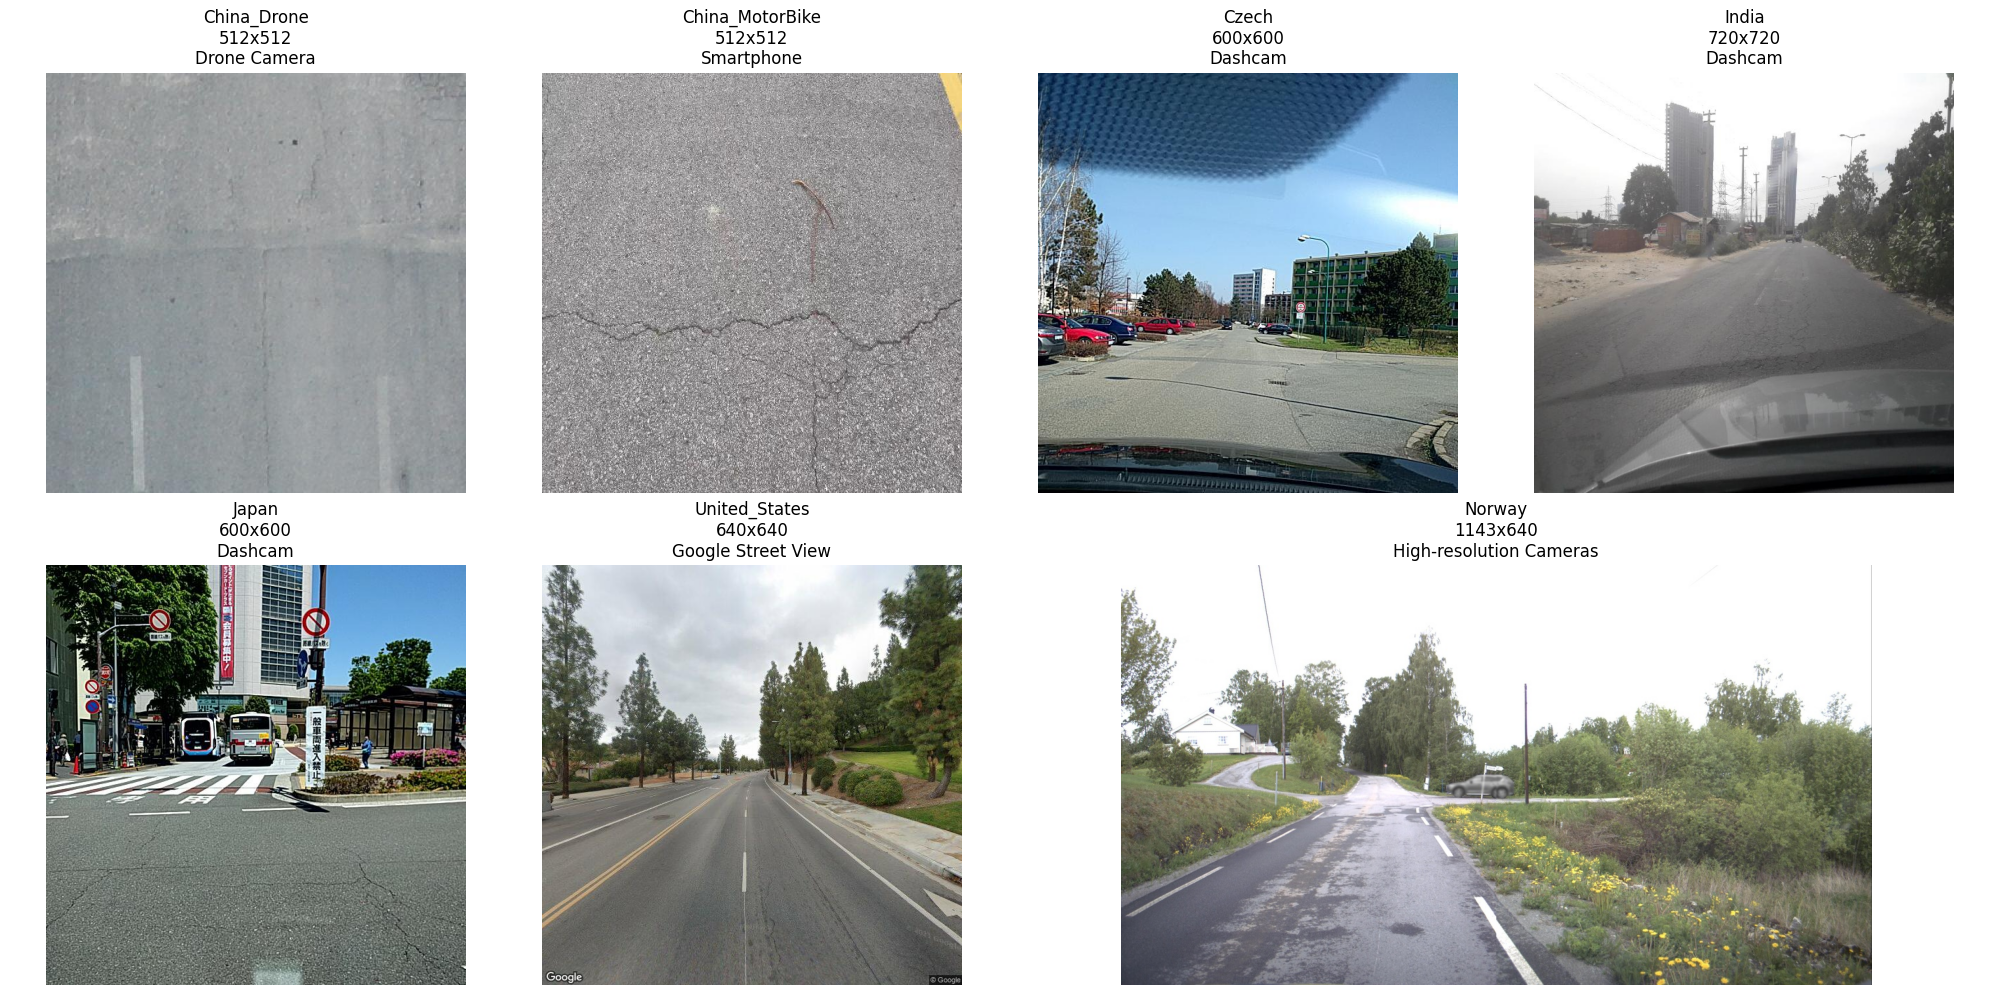
\includegraphics[width=1\textwidth]{img/example_images_regions.png}
    \caption{Ejemplos de imágenes de los datos de la CRDDC2022. Versión ampliada de la figura \ref{fig:example_images_region_large}.}
    \label{fig:example_images_region}
\end{figure}


\subsubsection{¿Cómo son las anotaciones?}
Las anotaciones como hemos dicho pueden venir en formato \texttt{xml} o \texttt{json} dependiendo de la fuente de descarga. No obstante, la información que contienen es la misma. Cada anotación contiene la información de su imagen correspondiente, y esta información se estructura de la siguiente forma:
\begin{itemize}
    \item \texttt{filename}: Nombre de la imagen.
    \item \texttt{size}: Tamaño de la imagen en píxeles.
    \item \texttt{objects}: Lista de objetos en la imagen. Cada objeto corresponde a un daño en el pavimento y contiene la siguiente información:
    \begin{itemize}
        \item \texttt{id}: Identificador de clase de daño de pavimento.
        \item \texttt{bndbox}: Coordenadas de la caja delimitadora del objeto.
    \end{itemize}
\end{itemize}
Es importante mencionar que las coordenadas de la caja delimitadora se proporcionan en formato \texttt{xmin, ymin, xmax, ymax}, donde \texttt{xmin} y \texttt{ymin} son las coordenadas del punto superior izquierdo de la caja, y \texttt{xmax} y \texttt{ymax} son las coordenadas del punto inferior derecho de la caja. Además, las coordenadas se proporcionan en píxeles. Los modelos YOLOv8 que vamos a utilizar requieren que las coordenadas de la caja delimitadora se proporcionen en formato \texttt{xcenter, ycenter, width, height}, donde \texttt{xcenter} y \texttt{ycenter} son las coordenadas del centro de la caja, y \texttt{width} y \texttt{height} son el ancho y alto de la caja. Además, las coordenadas deben estar normalizadas, es decir, deben estar en el rango $[0, 1]$. Por lo tanto, será necesario transformar las coordenadas de las anotaciones antes de entrenar los modelos.

Los datos originales contienen hasta 11 clases distintas de etiquetas de daños en el pavimento. Estas clases son: \texttt{D00, D20, D10, D40, D44, D50, D43, D01, D11, Repair, Block Crack}. No obstante, en la competición solo se consideran las cuatro primeras clases, que son las más comunes y resumen la mayoría de los daños en el pavimento. Estas clases tienen los siguientes significados:

\begin{itemize}
    \item \texttt{D00}: Longitudinal crack o \textit{grieta longitudinal}.
    \item \texttt{D10}: Transverse crack o \textit{grieta transversal}.
    \item \texttt{D20}: Alligator crack o \textit{grieta de cocodrilo}.
    \item \texttt{D40}: Pothole o \textit{bache}.
\end{itemize}

Las clases descartadas son: \texttt{D01} grietas longitudinales debido a una mala construcción de la junta longitudinal; \texttt{D11} grietas transversales debido a una mala construcción de la junta transversal; \texttt{D43} paso de peatones borrado; \texttt{D44} pintura borrada; \texttt{D50} tapa de alcantarilla; \texttt{Repair} reparación de pavimento; y \texttt{Block Crack} grieta en bloque. Algunas de estas clases se han fusionado con otras, como \texttt{D01} con \texttt{D00} o \texttt{D11} con \texttt{D10}. Otras clases se han descartado por no ser relevantes para la detección de daños en el pavimento, por falta de anotaciones o por no ser consistentes en todos los conjuntos de datos.

En la figura \ref{fig:example_damage_types} se pueden ver ejemplos de los tipos de daños en el pavimento de la CRDDC2022. Nótese que solo se han marcado los daños en el pavimento correspondientes a la clase que se quiere mostrar en cada imagen.

% Añadimos la imagen example_damage_types_h de la carpeta images
\begin{figure}[H]
    \centering
    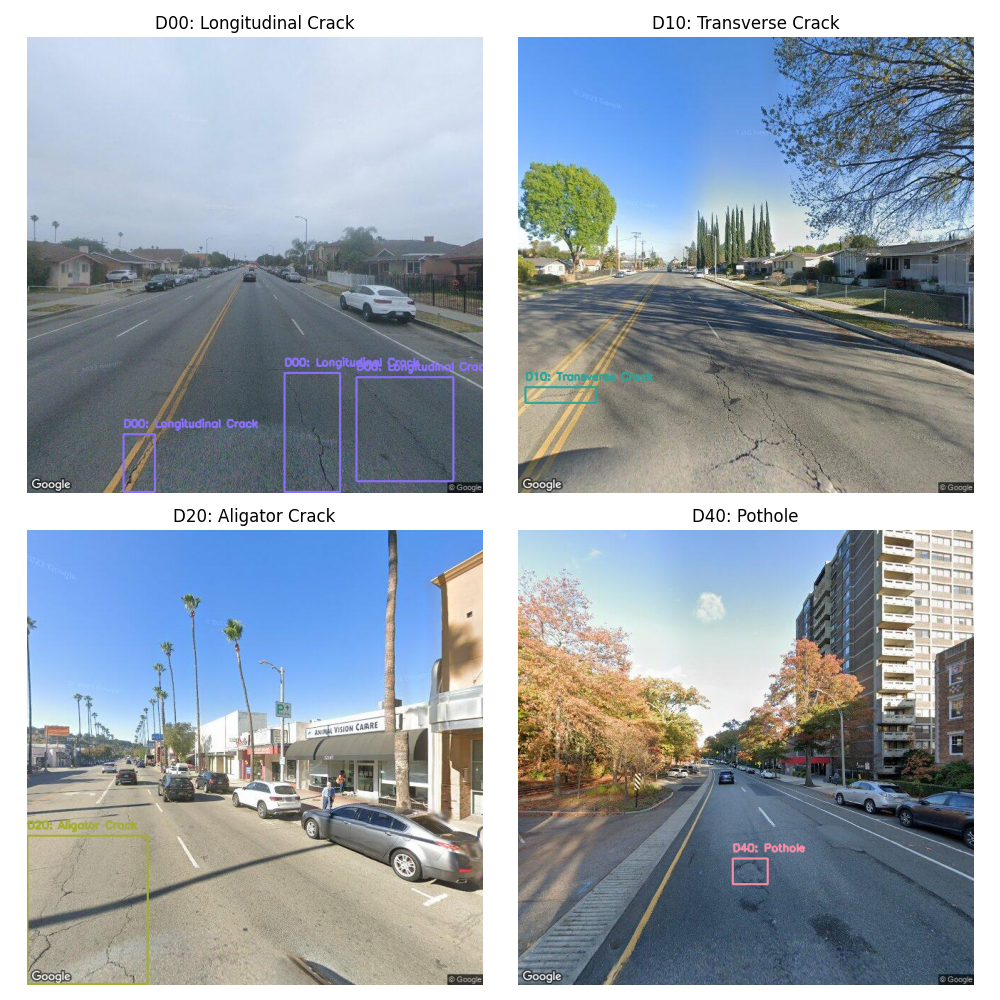
\includegraphics[width=0.85\textwidth]{img/example_damage_types_grid.png}
    \caption{Ejemplos de los tipos de daños en el pavimento de la CRDDC2022. Versión ampliada de la figura \ref{fig:example_damage_types_large}.}
    \label{fig:example_damage_types}
\end{figure}

El conjunto de datos descargado de DatasetNinja tiene la ventaja de agrupar todas las clases que se ignorarán en la competición en una sola clase llamada \texttt{Other Corruption}. Esto facilita el trabajo con los datos, ya que no es necesario realizar esta agrupación manualmente. En la figura \ref{fig:datasetNinja_class_count_bar} se muestra el número de anotaciones por clase en los datos de la CRDDC2022 y su desglose por región. La tabla \ref{tab:crddc2022_solutions} presenta los mismos datos en formato tabular. Se observa que la distribución de anotaciones por clase y región es muy desigual, con Japón teniendo una cantidad mucho mayor de anotaciones en comparación con regiones como China o la República Checa. Además, dentro de cada región, la distribución de anotaciones por clase también es dispareja, con regiones como India teniendo una alta proporción de Potholes y pocas grietas transversales, mientras que en Estados Unidos ocurre lo contrario. Esta desigualdad en la distribución de anotaciones por clase y región puede afectar el rendimiento de los modelos, llevando a un sobreajuste en favor de las regiones y clases más representadas. Este es un factor a considerar en futuras iteraciones del proyecto.

% Añadimos las gráficas daatasetNinja_class_count_bar y datasetNinja_class_count_by_region_bar como subfiguras
\begin{figure}[H]
    \centering
    \subfigure[Numero de anotaciones por clase]{
        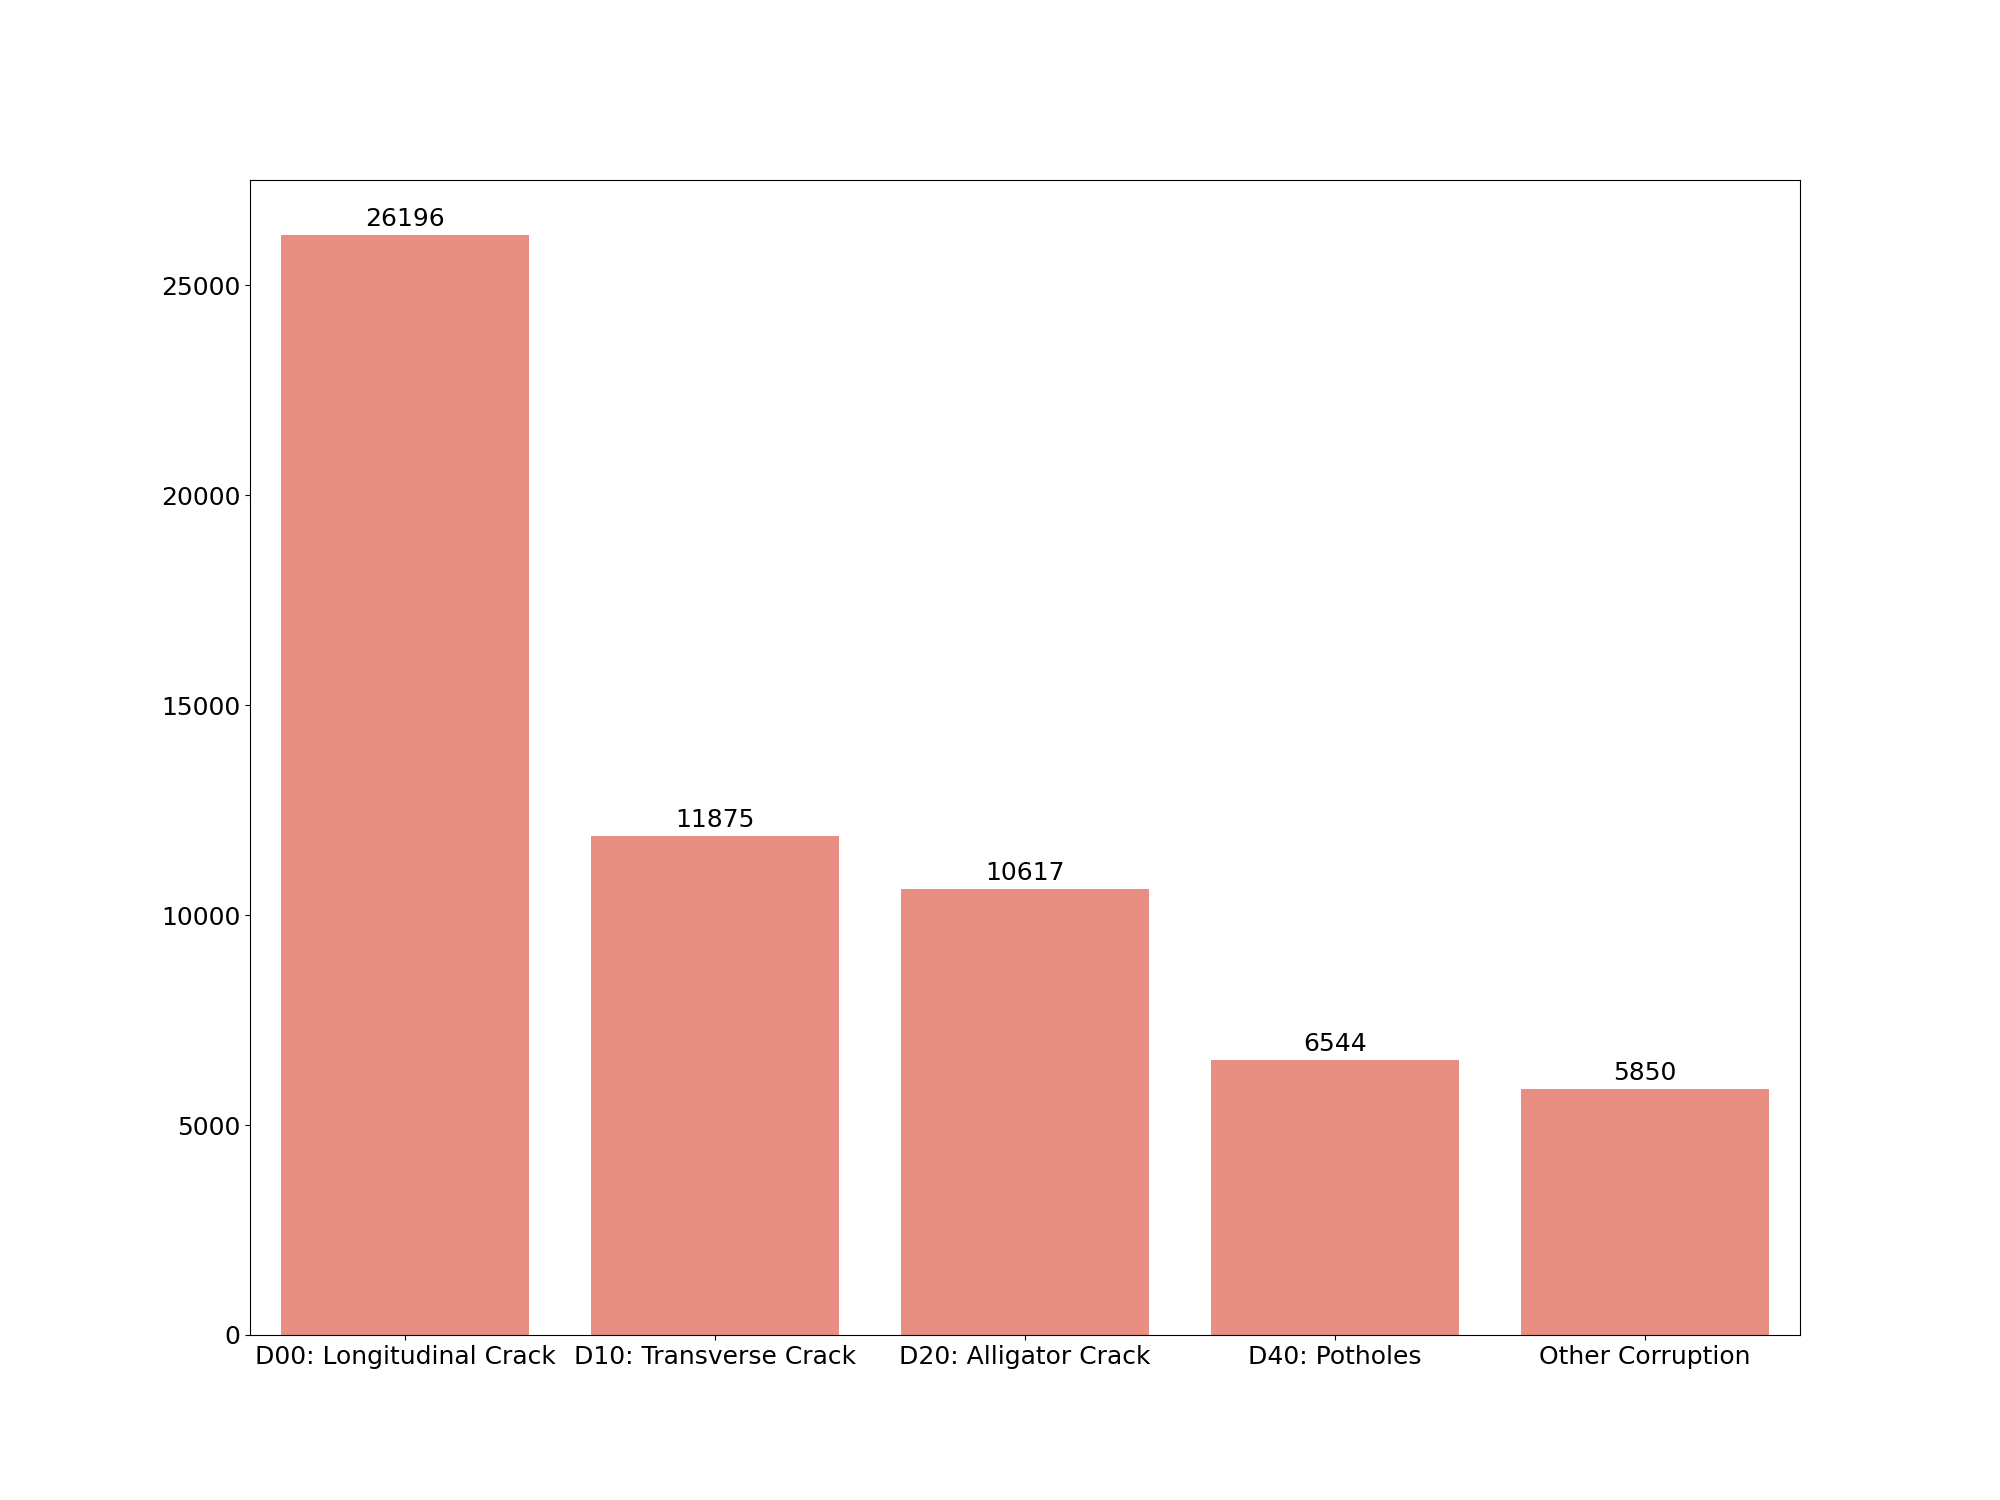
\includegraphics[width=0.45\textwidth]{../graphs/datasetNinja_class_count_bar.png}
        \label{fig:datasetNinja_class_count_bar_subfig1}
    }
    \subfigure[Numero de anotaciones por clase y región]{
        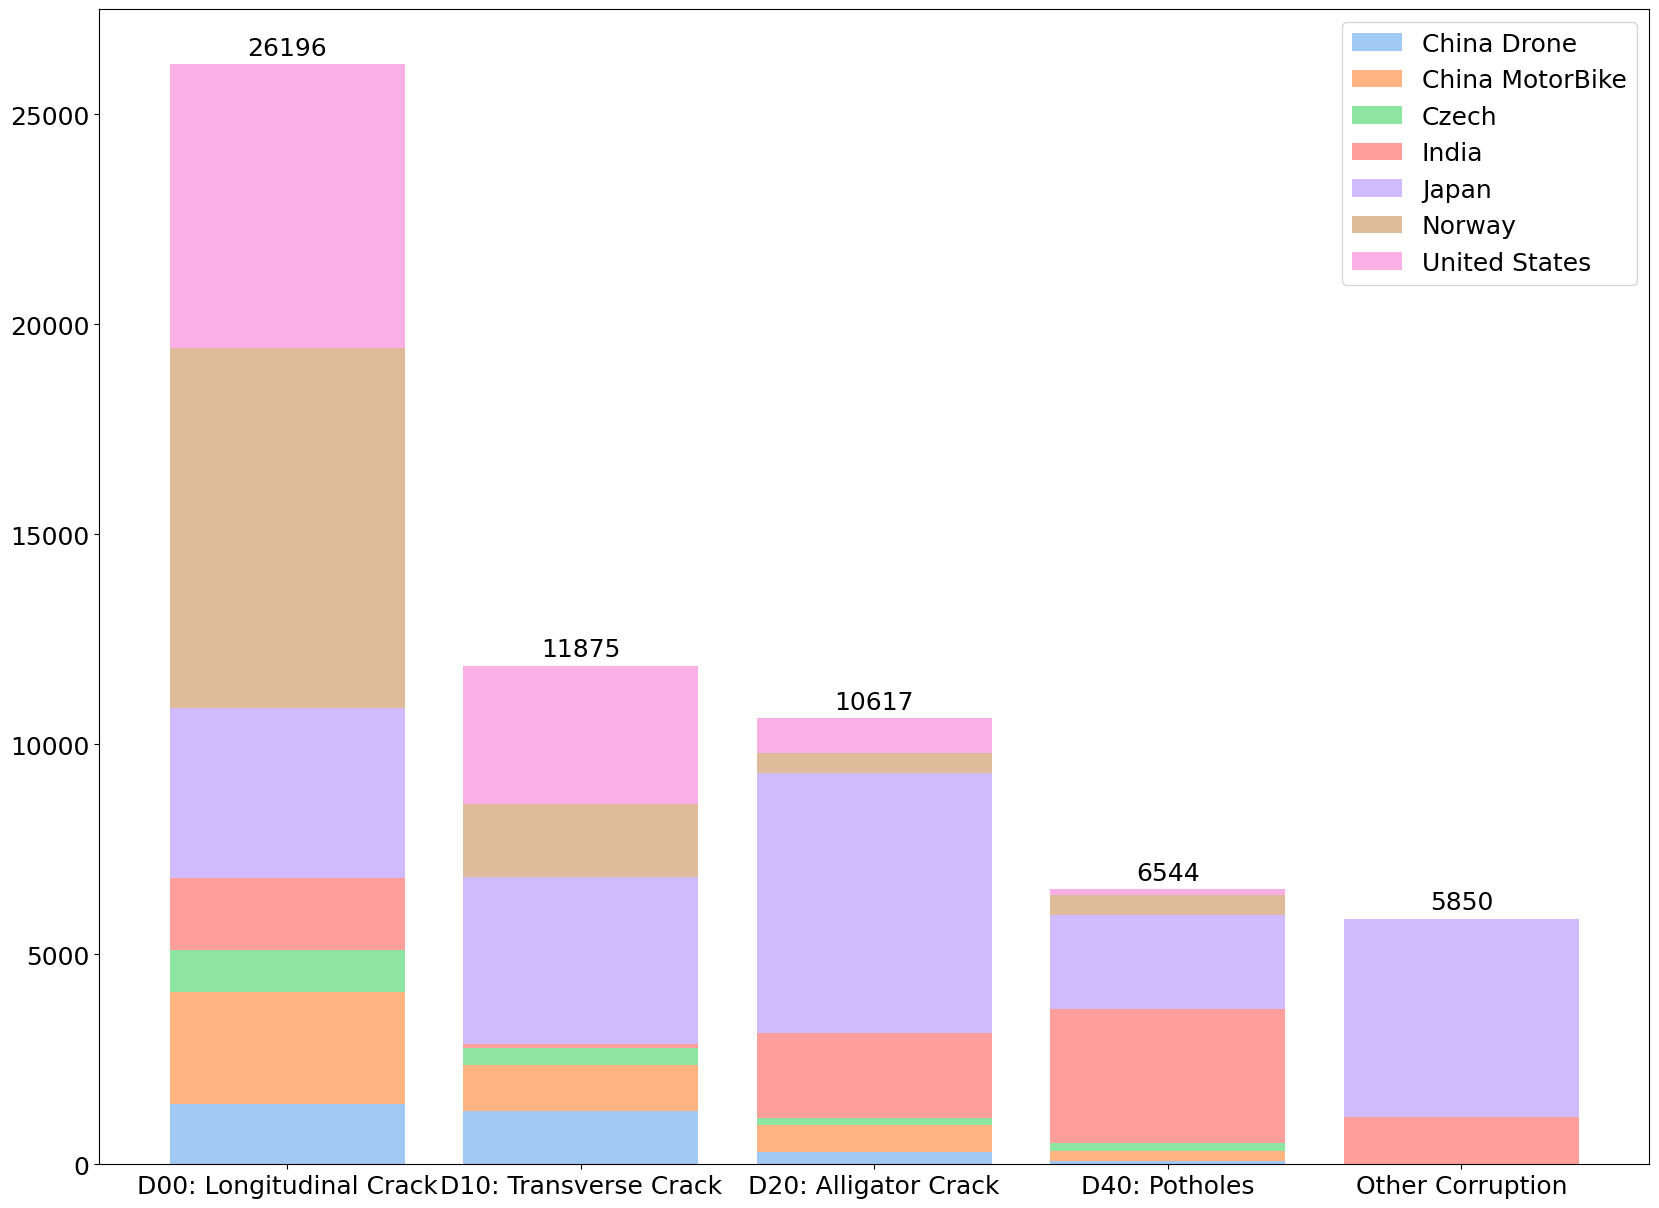
\includegraphics[width=0.45\textwidth]{../graphs/datasetNinja_class_count_by_region_bar.png}
        \label{fig:datasetNinja_class_count_bar_subfig2}
    }
    \caption{Número de anotaciones por clase en los datos de la CRDDC2022. Versión ampliada de la figura \ref{fig:datasetNinja_class_count_bar_large}.}
    \label{fig:datasetNinja_class_count_bar}
\end{figure}

\begin{table}[H]
    \centering
    \resizebox{\textwidth}{!}{
        \begin{tabular}{|l|r|r|r|r|r|r|}
        \hline
        \textbf{} & \textbf{D00: Longitudinal Crack} & \textbf{D10: Transverse Crack} & \textbf{D20: Alligator Crack} & \textbf{D40: Potholes}  & \textbf{Other Corruption} & \textbf{Total} \\ \hline
        \textbf{China\_Drone}       & 1426  & 1263  & 293   & 86    & 0     & 3068  \\ \hline
        \textbf{China\_MotorBike}   & 2678  & 1096  & 641   & 235   & 0     & 4650  \\ \hline
        \textbf{Czech}              & 988   & 399   & 161   & 197   & 0     & 1745  \\ \hline
        \textbf{India}              & 1735  & 113   & 2021  & 3187  & 1119  & 8175  \\ \hline
        \textbf{Japan}              & 4049  & 3979  & 6199  & 2243  & 4731  & 21201 \\ \hline
        \textbf{Norway}             & 8570  & 1730  & 468   & 461   & 0     & 11229 \\ \hline
        \textbf{United\_States}     & 6750  & 3295  & 834   & 135   & 0     & 11014 \\ \hline
        \textbf{Total}              & 26196 & 11875 & 10617 & 6544  & 5850  & 61082 \\ \hline
        \end{tabular}
    }
    \caption{Número de anotaciones por clase y región en los datos de la CRDDC2022.}
    \label{tab:anotaciones_por_clase_region}
\end{table}